\batchmode
\documentclass{beamer}
\usepackage[utf8]{inputenc}
\usepackage[ngerman]{babel}
\usepackage{amsmath}

\usetheme[deutsch]{KIT}
\author{Jan Haag (jan.haag@student.kit.edu)}
\title{Programmieren Tutorium 6 -- JCC, Referenzen, Listen}
\institute{Institut f\"{u}r Zeritfizierbare und Vertrauensw\"{u}rdige Informatiksysteme (ZVI)}
\TitleImage[scale=0.225]{frontpic.jpg}

\begin{document}
\begin{frame}
\maketitle
\end{frame}

\begin{frame}
\frametitle{Inhalt}
\tableofcontents
\end{frame}

\section{JCC, Kommentare}
\begin{frame}
\frametitle{JCC, Kommentare}
Siehe andere Folien...
\end{frame}

\section{Primitive Datentypen, Referenztypen}
\begin{frame}
\frametitle{Primitive Datentypen, Referenztypen}
\begin{description}
\item[primitive Datentypen]
\begin{itemize}
\item int
\item char
\item double
\item\dots
\end{itemize}
\item[Referenztypen]
\begin{itemize}
\item Arrays
\item Klassen
\item null
\end{itemize}
\end{description}
\end{frame}

\begin{frame}[fragile]
\frametitle{Unterschiede}
\begin{tabular}{l|l|l}
Operation & Primitive Datentypen & Referenztypen\\
\hline\\
\verb|=| & Wert & Referenz auf \emph{gleiches} Objekt\\
\verb|==| & Wertgleichheit & Referenzgleichheit\\
\verb|equals| & --- & Wertgleichheit\\
\end{tablular}\\
\vspace{1\baselineskip}
$\rightarrow$ boolean Object.equals(Object other)
\end{frame}

\section{Listen}
\begin{frame}
\frametitle{Listen}
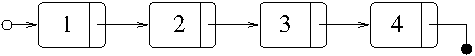
\includegraphics[scale=1.0]{list.pdf}
\end{frame}

\section{Aufgabe}
\begin{frame}[fragile]
\frametitle{Aufgabe}
Siehe Code.
\end{frame}

\begin{frame}
\frametitle{Ende}

\includegraphics[scale=0.4]{porn_folder.png}
\end{frame}
\end{document}
